%%-------------------------------------------------------------------------------------- Início
\section{Editor de Códigos}
\begin{frame}[allowframebreaks,fragile,t]{Preparação do Editor de Código}
  \begin{enumerate}
    
    \item Abre o terminal de linha de comandos e instale o conjunto de plugins do Gedit 
      que emulam o TextMate.
    \begin{lstlisting}[style=BashInputStyle]
      $ sudo apt-add-repository ppa:ubuntu-on-rails/ppa
      $ sudo apt-get update
      $ sudo apt-get install gedit-gmate
    \end{lstlisting}
    
    \item Abra o editor de texto teclando \verb!ALT+F2!, digite "gedit" e, por último,
      clique duas vezes no ícone do editor \alert{GEdit}.
    
    
    \item Clique no menu \alert{Edit} e escolha a opção \alert{Preferences}.
    \begin{itemize}
      \item na aba \alert{View}, configure e selecione as opções abaixo.
      \begin{figure}[h!]
	\centering
	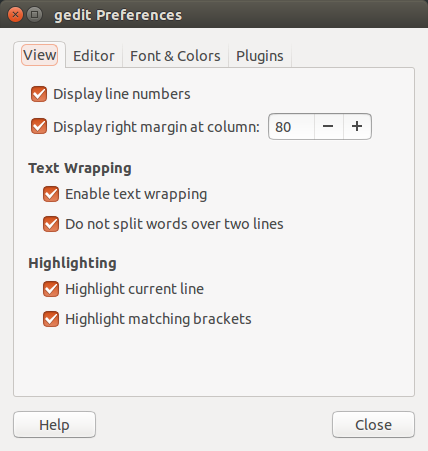
\includegraphics[width=0.30\textwidth]{devops/imagens/gedit-1.png}
      \end{figure}
    \end{itemize}

    \framebreak
    \begin{itemize}
      \item na aba \alert{Editor}, configure e selecione as opções abaixo.
      \begin{figure}[h!]
	\centering
	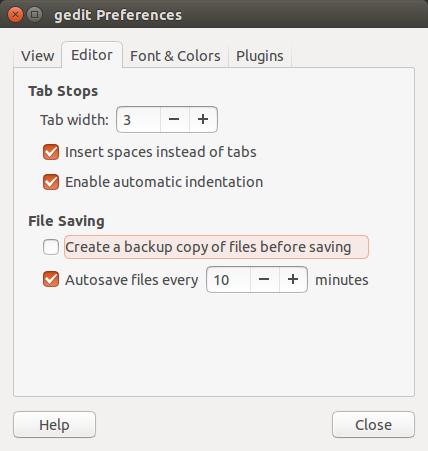
\includegraphics[width=0.30\textwidth]{devops/imagens/gedit-2.png}
      \end{figure}
    \end{itemize}

    \framebreak
    \begin{itemize}
      \item na aba \alert{Fontes \& Colors}, configure e selecione as opções abaixo.
      \begin{figure}[h!]
	\centering
	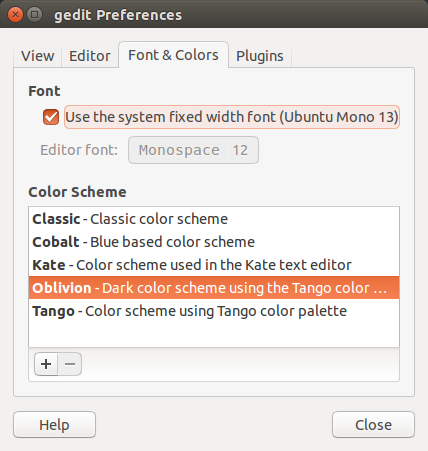
\includegraphics[width=0.30\textwidth]{devops/imagens/gedit-3.png}
      \end{figure}
    \end{itemize}

    \framebreak
    \begin{itemize}
      \item na aba \alert{Plugins}, selecione \alert{File Browser Pane}.
      \begin{figure}[h!]
	\centering
	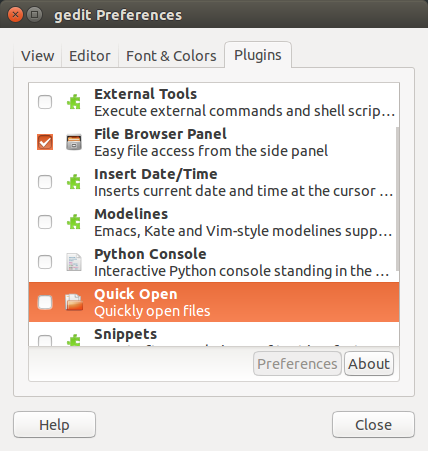
\includegraphics[width=0.30\textwidth]{devops/imagens/gedit-4.png}
      \end{figure}
    \end{itemize}
    
    \item Finalmente, clique no botão \verb!Close!.
      
    \end{enumerate}
\end{frame} 
